%!TeX root=../main.tex

% TODO: 
%   - Update activation pic


\begin{figure}[h!]        
\vskip -0.05in % useful knobs to optimize layout
    \centering        
    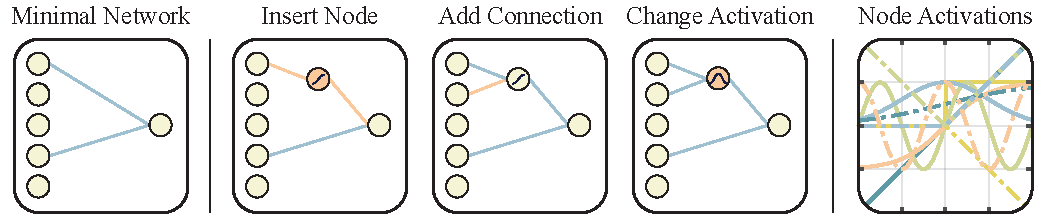
\includegraphics[width=1\textwidth]{img/topOper.pdf}  
\vskip -0.05in % useful knobs to optimize layout
    \caption      
    {     
        \textit{Operators for Searching the Space of Network Topologies}
        \newline
        \textit{Left:} A minimal network topology, with input and outputs only partially connected. 
        \newline
        \textit{Middle:} Networks are altered in one of three ways. \textit{Insert Node}: a new node is inserted by splitting an existing connection. \textit{Add Connection}: a new connection is added by connecting two previously unconnected nodes. \textit{Change Activation}: the activation function of a hidden node is reassigned.
        \newline % DH: added for readabiliy
        \textit{Right:} Possible activation functions (linear, step, sin, cosine, Gaussian, tanh, sigmoid, absolute value, invert (i.e. negative linear), ReLU) shown over the range $[2,2]$.
        }         
    \label{fig:topsearch}   
\vskip -0.05in % useful knobs to optimize layout
\end{figure}